% !TEX root = ../my-thesis.tex
%

\chapter{Benchmark}
\label{sec:Benchmark}

\cleanchapterquote{Un petit chapitre pour le doctorant, un grand chapitre pour l'humanité}{Doctorant anonyme}{(Citation temporaire)}

\section{Propriétés}
\label{sec:Benchmark}

Dans cette section, nous abordons la conception d'un banc d'étude permettant l'étude des filtres de rehaussement. Celui-ci nécessite de comprendre le fonctionnement des filtres de manière fine afin que leur comparaison soit faite de manière la plus fiable possible.

La comparaison de filtres basée uniquement sur la littérature n'est pas un moyen fiable de se forger une opinion sur quel filtre choisir pour une application spécifique. Il faut donc tester ceux-ci en pratique.

\subsection{Filtres}
\label{sec:Filtres}

Former une base homogène de filtres n'est pas une tâche simple. Celle-ci nécessite la recherche de code existant ou l'implémentation à partir de l'article original.

L'implémentation à partir de l'article original peut-être rendue complexe par un manque de détail ou de clarté de la part de l'auteur qui doit souvent se soumettre à un exercice de concision. Celle-ci peut aussi survenir d'une difficulté de compréhension de la part du lecteur. En particulier lorsque les articles sont écrits dans une langue étrangère. 

La collecte d'implémentations existantes n'est pas non plus évidente. En effet, il est possible que plusieurs versions existent. Il est alors nécessaire de vérifier le code en détail. Celles-ci peuvent présenter des interfaces différentes de l'article original et nécessiter un travail de translation d'une interface à l'autre. Certains codes sont disponibles mais ont une dette technologique importante suite à l'évolution des logiciels ou des librairies nécessaires à leur fonctionnement. Enfin, la mutiplicité des languages, librairies et logiciels sur lesquels sont déployés les filtres ajoute au temps dédié à cette tâche. Enfin, ce travail est souvent réalisé de manière isolée par un doctorant, un chercheur ou stagiaire pour leurs expériences et ne profite pas à la prochaine personne travaillant sur le sujet et qui doit reprendre de lui même la totalité de cette recherche.

Dans ces travaux, nous avons sélectionné, adapté et implémenté sept filtres qui répondaient tous à une problématique spécifique du rehaussement TABLE~\ref{Tab:available_vesselness}. La diversité de leur origine est résumée dans la table TABLE~ \ref{Tab:origins_vesselness}. Il a été choisi d'implémenter ces filtres et leurs modifications en C++ avec la librairie ITK. Le C++ est particulièrement connu pour sa rapidité, crucial pour des applications 3D. La librairie open source ITK (insight toolkit), développée par Kitware Inc. depuis 2001, est la plus grosse librairie de traitement d'images médicales. Elle fournit un ensemble de briques algorithmiques déjà implémentées et a l'avantage de lire nativement une grande diversité de formats d'images médicales ce qui est un atout la diffusion de notre banc de test.

Cette librairie a une communauté active et connait des mises à jours régulières.

\begin{table}
    \begin{center}
  \begin{tabular}{l|l|l}
  Méthode   &  Idée centrale                                                                       & Date \\ \hline  \hline 
  Sato      & Reconnexion des vaisseaux, contrôle du bruit                                         & 1997 \\ \hline
  Frangi    & Contrôle sur l'atténuation des structures en plateau et en blobs                     & 1998 \\ \hline
  Meijering & Détections de fines structures allongées                                             & 2004 \\ \hline
  OOF       & Limitation du débordement des réponses lié à l'espace d'échelle gaussien             & 2010 \\ \hline
  Jerman    & Contrôle de l'homogénéité des réponses des vaisseaux                                 & 2016 \\ \hline
  Zhang     & Pré-traitement pour limiter le rehaussement des bordures du foie (TDM foie)          & 2018 \\ \hline
  RORPO     & Détection par chemins et différentiation des vaisseaux par vote sur les orientations & 2018  
  \end{tabular}
  \end{center}
  \caption{Méthodes disponibles et idées principales guidant leurs conceptions}
  \label{Tab:origins_vesselness}
  \end{table}

  \begin{table}
    \begin{center}
        \begin{tabular}{l|l|l|l}
            Méthode   &  Provenance                                     & Etat \\ \hline  \hline 
            Sato      & librairie ITK (C++)                             & prêt à l'emploi \\ \hline
            Frangi    & librairie ITK (C++)                             & prêt à l'emploi \\ \hline
            Meijering & Github (Matlab), scipy                          & pondération proposée étrange  \\ \hline
            OOF       & Site de l'auteur (Matlab), insight journal (C++)& obsolète \\ \hline
            Jerman    & Github de l'auteur (Matlab)                     & prêt à l'emploi \\ \hline
            Zhang     & Non disponible                                  & non implémenté \\ \hline
            RORPO     & Github de l'auteur (C++)                        & prêt à l'emploi  
        \end{tabular}
    \end{center}
    \caption{Origine des méthodes}
    \label{Tab:origins_vesselness}
  \end{table}

La conception de notre banc de test a été guidé par plusieurs axes majeurs.
  
Le premier axe de conception a été d'évaluer le rehaussement pour la segmentation de voxélique. Nous aurions pu envisager l'étude du rehaussement pour d'autres types de segmentation comme l'extraction de la ligne centrale. Cependant la nature des vérités terrains disponibles et une plus grande quantité d'applications annexes de la segmentation voxélique nous a conforté dans ce choix.

Le rehaussement de vaisseaux est parfois présenté comme une carte chaleur ou de probabilité, où, pour chaque voxel on associe une quantité d'appartenance à un vaisseau. Pour le filtre de Frangi cette quantité est définie entre 0 et 1. Cette propriété est désirable dans de nombreuses applications, car plus simple à manipulier que des filtres définis sur des domaines plus larges.

Cependant, la réponse de tous les filtres ne partage pas nécessairement cette propriété. Par design seuls Jerman et Zhang possèdent cette propriété. La réponse de Sato est définie sur $[0,+\infty]$, tout comme celle d'OOF et de Meijering. RORPO est un cas particulier, car l'intensité de sortie du filtre dépend de l'intensité maximum de l'image source. En effet, RORPO se base sur des ouvertures morpholo 

Dans une optique de généralisation et de diffusion des filtres, nous partons du principe que les images des bases de données ne sont pas normalisées. Il faut donc contraindre les sorties des filtres entre zéro et un. Nous avons choisi pour Sato, OOF et Meijering de normaliser la réponse de sortie en fonction de la plus grande valeur de sortie du filtre $ \frac{I_{rehaussement}(x)} {max(I{rehaussement}(x))} $. Pour RORPO dont la sortie est liée à l'intensité de l'image d'entrée la normalisation prend la forme $ \frac{I_{rehaussement}(x)} {max(I(x))} $.

A noter que des variantes d'implémentations existent et une attention particulière doit être portée aux types d'images pris en charge par les algorithmes. En effet, la dynamique des images médicales n'est pas commune.
Une image 2D est souvent représentée sur 8 bits exprimant 256 niveaux de gris $[0,255]$ (multiplié par 3 canaux pour les images couleurs). Les images médicales possèdent la plupart du temps un seul cannal avec parfois une dynamique de niveaux de gris plus importante de 16 ou 32 bits et peuvent présenter des valeurs négatives.

Il faut donc s'assurer que les filtres supportent les images. Par exemple, RORPO ne supporte que des valeurs de pixels positifs et nécessite de faire une translation des niveaux de gris négatifs sous peine d'obtenir des comportements non définis.

Il peut souvent être utile de ne traiter qu'une partie de l'image, par exemple lorsqu'un ne veut rehausser les vaisseaux que d'un organe en particulier. La manière la plus simple est de définir un masque binaire de la même taille que l'image où l'on renseigne pour chaque voxel s'il appartient à la zone à traiter (1 ou 255) ou s'il appartient à la zone à ne pas traiter (0). Là encore, il faut être attentif à l'implémentation du masque. Une première implémentation consiste appliquer le masque sur le rehaussement après coup. Le filtre est appliqué à toute l'image avant de ne conserver que la partie concernant à l'organe observé. Cette implémentation a le désavantage de calculer du rehaussement dans des zones non utilisées par la suite.Une seconde implémentation consiste à masquer l'image dans un premier temps, puis de calculer le rehaussement dans cette image masquée. On gagne ainsi du temps de calcul dans les zones à zéro. Cependant, cette méthode créé artificiellement de faux rebords avec un différentiel d'intensités marqué.

De plus, on peut classer les filtres de rehaussement en deux catégories. Les filtres à seule information locale et les filtres à information locale et globale.

Les filtres à information locale sont Frangi, Sato, RORPO, OOF. Ceux-ci ne considèrent le rehaussement que par rapport à des mesures effectuées dans un voisinage local défini par la taille de la gaussienne pour les méthodes à espace d'échelles gaussien et par la taille de l'élément structurant pour RORPO.

Les filtres à information globale sont Meijering, Jerman et Zhang.

Meijering et Jerman/Zhang nécessitent respectivement la plus faible et la plus grande valeur propre de la zone sur lequel est appliqué le rehaussement. Le pré-filtrage de Zhang nécessite lui aussi une information globale puisque son pré-filtrage repose sur la classification de l'ensemble des pixels de la zone de rehaussement.

Dans le cas de ces filtres, une implémentation naive des masques à un impact critique sur le résultat du rehaussement. En effet, une image de l'abdomen contient aussi les os de la cage thoracique qui possèdent une intensité largement supérieurs aux vaisseaux du foie. Dans le cas d'un filtre à information globale comme le filtre de Jerman, la mesure de rehaussement sera pondérée par les valeurs propres maximales de l'image, donc celle des os, et non celles des vaisseaux. 

Une stratégie de masque a donc été choise spécifiquement pour chaque masques. Ainsi pour Frangi, Sato, OOF, RORPO le masque est appliqué après le rehaussement, cela afin de limiter l'introduction de faux gradients liés au masque.

\begin{figure}
  \centering
  \includegraphics[height=3cm]{Images/img_required.jpg}
  \label{fig:mask_intensity_profile}
  \caption{profil d'intensité avec et sans masque. Le masque exacerbe la démarcation}
\end{figure}

Nous avons implémenté nous même les filtres de Jerman, Meijering et Zhang nous permettant d'avoir un contrôle plus fin sur l'étape d'application du masque. Afin de combiner les deux propriétés de limitation du temps de calcul et de non introduction de bordures nettes artificielles, l'opération de masque est introduite entre le calcul de la matrice hessienne et le calcul de ses valeurs propres. Ne sont calculées les valeurs propres que des pixels appartenants au masque. On obtient ainsi le meilleur entre masque en amont et masques en aval.

\begin{figure}
  \centering
  \includegraphics[height=3cm]{Images/img_required.jpg}
  \label{fig:smart_mask_effect}
  \caption{Effet d'un masque intelligent sur Jerman vs sans masque.}
\end{figure}

\tikzstyle{startstop} = [rectangle, rounded corners, minimum width=3cm, minimum height=1cm,text centered, draw=black, fill=lightgray!30]
\tikzstyle{stepNode} = [circle, minimum width=1cm, minimum height=1cm, text centered, draw=black, fill=white!30]
\tikzstyle{process} = [rectangle, minimum width=3cm, minimum height=1cm, text centered, draw=red, fill=white!30]
\tikzstyle{arrow} = [thick,->,>=stealth]

\begin{figure}[!t]

    \centering
    %\resizebox{\linewidth}{
      
  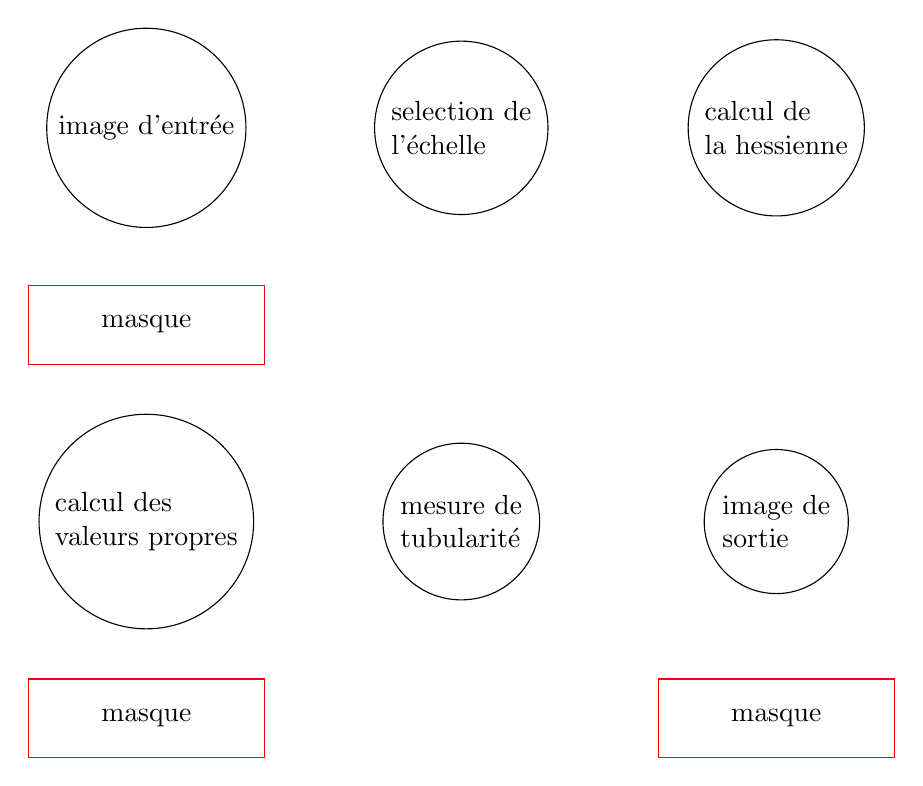
\begin{tikzpicture}[node distance=2cm]
    \node (input)[stepNode] {image d'entrée};
    \node (scale_selection)[stepNode, right of=input,xshift=2cm,align=left] {selection de \\ l'échelle};
    \node (hessian)[stepNode, right of=scale_selection,xshift=2cm,align=left] {calcul de \\ la hessienne};
    \node (EV)[stepNode, below of=input,yshift=-3cm,align=left] {calcul des \\ valeurs propres};
    \node (vesselness)[stepNode, right of=EV,xshift=2cm,align=left] {mesure de \\ tubularité};
    \node (output)[stepNode, right of=vesselness,xshift=2cm,align=left] {image de \\ sortie};

    \node (p1)[process,below of=input,yshift=-0.5cm]{masque};
    \node (p2)[process,below of=EV,yshift=-0.5cm]{masque};
    \node (p3)[process,below of=output,yshift=-0.5cm]{masque};
    
    % \draw [arrow] (bestIntrinsicParameter) -- (bestParameters);
    % \draw [arrow] (bestScaleParameter) -| node[anchor=east]{}([shift={(1.3cm,0mm)}]bestScaleParameter.east)|-([shift={(0mm,-1mm)}]computeParams2.west);
  \end{tikzpicture}
%}
\caption{Emplacement possibles pour masquer la réponse. Chaque emplacement possède un avantage}
\label{FIG:masks_posible_location}
\end{figure}

Zhang est le filtre le plus complexe, avec une étape de pré-traitement avec un K-moyenne paramétrant un filtrage par sigmoid et la mesure de rehaussement. Dans la méthode originale, le nombre de classes du K-moyenne est défini par rapport à des images masquées. Ce K-moyenne est donc appliqué sur l'image globale masquée (fond mis à 0) avant le filtrage par sigmoid. Ensuite la même stratégie de masquage que Jerman et Meijering est utilisé.Le K-mean classique est une opération coûteuse, en particulier lorsqu'il est effectué sur un volume 3D. Afin d'éviter un surcoût nous avons utilisé un K-mean à partir d'un quadtree qui réduit significativement le temps de calcul de cette étape.



Les 7 filtres sont implémentés en C++ et reposent sur la librairie ITK. Ceux-ci sont implémentés sont forme de CLI (command line interface) indépendants du cadre du banc de test et peuvent être utilisés indépendamment de celui-ci. Cela veut aussi dire que n'importe quel nouveau filtre respectant l'interface définie dans le benchmark (c'est à dire une entrée, une sortie et un masque optionnel) peut être ajouté de manière transparente à celui-ci.

\subsection{Pré-traitements des jeux de données}
\label{sec:Benchmark:traitement_des_données}

Pour évaluer la segmentation voxélique de manière précise, nous avons souhaité évaluer le rehaussement dans plusieurs régions. La première région est l'organe dans sa totalité. Cette région est celle choisis la plupart du temps pour la segmentation. L'étude de cette région pose plusieurs questions. Un filtre arrive t'il à rehausser les vaisseaux sans rehausser d'autres éléments de l'image ? Dans quelle proportion ? Le rehaussement introduit'il de nouvelles structures ou artefacts ?

La seconde région d'intérêt concerne les vaisseaux et leur voisinage. Cette région nécessite la segmentation manuelle des vaisseaux par un expert. Elle permet de répondre à plusieurs questions ? Quelle est la qualité du rehaussement des vaisseaux ? Les vaisseaux sont-ils rehaussés avec une taille supérieure ou inférieure à leur taille réelle ? Cette Région peut-être subdivisée en partitions en fonction de la taille ou de la hiérarchie des vaisseaux. On peut par exemple différencier le rehaussement des petits vaisseaux et des gros vaisseaux.

La troisième région d'intérêt concerne les bifurcations des vaisseaux. Ces zones sont particulières car elles conrespondent à une jonctions des vaisseaux tubulaires. La géométrie n'est plus tubulaire dans ces zones. Le rehaussement peut donc être affaiblit dans ces zones. Cette perte de signal a été notée dans de nombreuses publications, le plus souvent de manière visuelle sur des données synthétiques.

En effet, le rehaussement n'est jamais homogène et produit des résultats différents en fonction du rehaussement recherché.

La construction de ces zones d'intérêts est parfois complexe à réaliser. La géométrie des organes est relativement simple et peut se faire à l'aide d'outils semi automatiques comme les levels sets, ou la croissance de région à partir de marqueurs placés à la main. Le mouvement du patient durant l'acquisition peut faire fusionner des tissues, comme c'est souvent le cas entre le foie et l'estomac. Dans ce cas, une correction manuelle peut-être nécessaire.

Pour la vérité terrain des vaisseaux, une première approximation peut-être obtenue par seuillage, cependant la majeure partie des données doit être réalisée par un expert. Une paire de vue 2D et MIP 3D permettent de valider les annotations de manière simple et améliorent considérablement la qualité des annotations. Pour obtenir une vérité terrain des vaisseaux et de leur voisinage, il suffit de dilater la vérité terrain des vaisseaux.

Nous avons dans un premier temps réalisé une dilatation globale. Cependant, celle-ci n'est pas forcément pertinente selon la taille des vaiseaux, puisque les gros vaisseaux se retrouvent avec une proportion vaisseaux/fond inférieure aux petits vaisseaux. De plus, afin d'avoir une information complémentaire sur le voisinage des vaisseaux, nous avons réalisé une partition par taille en 3 classes : Gros vaisseaux, un tronc portal ou des artères alimentant le cercle de Willis. Les vaisseaux de taille moyennes, vaisseaux principaux dans les organes, les vaisseaux de petite taille.

Cette partition nécessite une traitement sur la vérité terrain originale. Celle-ci nécessite de labéliser chaque branche de vaisseaux en fonction de leur diamètres avant de les classifier dans trois sous labels.

\paragraph{Génération de données synthétiques}

Nous avons à notre disposition la base de donnée de l'Ircad pour le foie. Cependant cette base est acquise par tomodensitométrie. Hors, cette modalité a été relativement bien explorée dans la littérature et l'un des objectifs initial était l'évaluation du rehaussement dans des images IRM. Le manque de données IRM annotées nous oblige à nous tourner vers des données synthétiques. Les bases de données synthétiques ont l'inconvénient d'être moins réalistes que les bases naturelles. Elles présentent cependant l'avantage d'un environnement complètement contrôlé par l'utilisateur et permettent d'obtenir des vérités terrains au pixel prêt.
\todo{voir si vascusynth est a présenter ici ou dans le chapitre 2, base de données}

Vascusynth, présenté dans le Chapitre 2, permet de définir des images synthétiques. Le logiciel permet de créer un arbre vasculaire en précisant le nombre d'extrémités de celui-ci, une carte d'oxygénation contrôlant les zones où peut s'étendre l'arbre vasculaire et une suite de paramètres dont la pression sanguine à l'origine.

Nous avons utilisé dans nos expériences la base de donnée de 2013 disponible sur le site de vascusynth. Cette base est composée de volumes avec des arbres vasculaires de différentes tailles sur un fond nul. VascuSynth produit des images en niveau de gris de 0 à 255. L'intensité des vaisseaux est relativement forte (autour de 230, à vérifier) et n'est pas homogène. L'intensité des vaisseaux décroit légèrement sur les bords de ceux-ci et est un peu plus faible pour les petits vaisseaux.

On peut obtenir une vérité terrain au pixel prêt en binarisant ce volume initial.

Nous avons voulu transformer ces images de manière à imiter l'apparance de l'IRM appliqué au foie. Cette génération de volumes IRM a connu plusieurs itérations que nous détaillons ici.

% intensité du foie
Nous avons généré nos images en 4 étapes.
Premièrement, nous avons redéfini la game d'intensité des vaisseaux. En effet, ceux-ci étant d'intensité trop élevés, ils ne permettent pas l'ajout de bruit et d'éléments additifs sans saturer les voxels et perdre l'information des vaisseaux. Une simple mise à l'échelle des intensités et une translation suffisent. Ensuite, nous avons ajouté un fond homogène d'intensité égale à l'intensité minimale des vaisseaux. En effet, dans l'imagerie du foie avec agent de contraste, les vaisseaux sont en principe d'intensité supérieure ou égale à l'intensité des tissus.


Dans un premier temps, nous n'avons pas réalisé de changement d'intensité le long des vaisseaux. Nous aurions pu faire décroitre l'intensité des vaisseaux en partant de la base de l'arbre et en faisant décroitre la valeur des voxels des vaisseaux par propagation de proche en proche. Cependant, les variations d'intensités dans les vaisseaux est un processus plus complexe qu'une simple baisse linéaire de l'intensité. Cette variation dépend des propriétés de mécaniques des fluides de l'agent de contraste dans le sang ainsi que de la géométrie des vaisseaux.


Nous avons ensuite voulu exploiter les différences d'intensité entre les tissus de même nature. Nous émulons cette non homogénéité illustrée dans le Chapitre 2, par la création d'un volume dans lequel 3 gaussiennes de taille $sigma=40$ sont tirés dans l'espace de manière aléatoire. Un opérateur max est ensuite utilisé entre le volume contenant les vaisseaux et les gaussiennes d'intensité similaire. L'opérateur max avait été choisi de manière à émuler l'intensité des vaisseaux les plus fins qui se fondent dans l'intensité des tissues environnants.


Nous avons ensuite ajouté du bruit ricien qui est un bruit multiplicatif spécifique à l'IRM. Par contraste, la plupart des expériences sur bases de données synthétiques appliquent une mixture de bruit de poisson et gaussien caractéristique du bruit présent en tomodensitométrie.

Cette première itération était une bonne approximation. Cependant celle-ci souffre de plusieurs limitations. Premièrement la dynamique d'intensité est établie de manière visuelle. De même pour le bruit ricien. deuxièmement, le max effectué entre les images et les vaisseaux fait disparaitre des vaisseaux qui sont tout de même présents dans la vérité terrain. On introduit ainsi une baisse artificielle des performances puisque qu'aucun filtre n'est en réalité capable de rehausser ces structures invisibles. En vérité, la pupart des vaisseaux peuvent être récupérés par un seuillage simple lorsque le niveau de bruit ne recouvre pas le signal. Ce problème est notamment visible à travers les MIP puisque l'intégralité des vaisseaux sont visibles quand ils ne sont pas recouverts par des blobs gaussiens.

Dans une deuxième itération nous avons revu le processus de création de ces volumes.

Les vaisseaux sont toujours mis à l'échelle et le fond toujours définit comme l'intensité minimale des vaisseaux. Cependant, la plage d'intensité des vaisseaux est cette fois ci définit par rapport à des mesures faites sur des bases de données réelles. Pour cela nous avons réalisé des mesures manuelles sur des images d'IRM. Sur quelques volumes (de mémoire 5-6, retrouver les valeurs), une dizaine de coupes axiales ont été réalisée sur lequelles ont été annotés deux masques, un masque des tissues et un masque des vaisseaux. Pour chaque type de masque, nous avons calculé la moyenne et l'écart type de l'intensité des vaisseaux et des tissues du foie. La moyenne des tissues du foie est de 1273 contre 1400 pour celle des vaisseaux. L'écart type respectif des tissues est de 144 et de 189 pour les vaisseaux pour des volumes avec une dynamique d'intensité comprise entre 0 et 3000. En exprimant ces quantités proportionnellement à la dynamique de vascusynth ($[0,255]$), on obtient $\mu=108 \pm 12$ pour les tissues du foie et $\mu=119 \pm 16$. En pratique le différentiel entre la moyenne des vaisseaux et des tissues est faible, alors qu'elle est localement plus importante. Cet écart est aussi trop faible pour obtenir des gaussiennes discrètes avec un sigma élevé de bonne qualité dans les étapes suivantes. Nous avons donc considéré l'intensité des vaisseaux comme la somme de leur moyenne et de l'écart type. Nous augmentons ainsi la dynamique tout en restant cohérent avec les mesures physiques.

Nous avons ensuite introduit deux filtres d'inhomogénéité : Un premier afin de diversifier le profil d'intensité des vaisseaux et un second pour diversifier l'intensité globale de l'image. Dans le premier cas, celle-ci essait d'approcher les variations d'intensités lié à l'agent de contraste. Dans le second cas, cette modification a été faite pour que le jeux de donnée soit résistant à une segmentation par simple seuillage. L'objectif est alors que localement, les vaisseaux restent des maxima locaux mais que ceux-ci soient d'intensité plus faible que des tissues du foie situés à l'autre bout du volume.

Pour cela l'algorithme de génération change légèrement. Pour le changement d'intensité dans les vaisseaux, on utilise un masque avec des gaussiennes tirées aléatoirements, ces gaussiennes sont pondérées de manière à faire diminuer l'intensité des vaisseaux au maximum de $30\%$ par rapport à leur intensité initiale. Les gaussiennes étant tirées dans l'espace entier de l'image on obtient des variations non linéaires le long des vaisseaux.

Cette étape est réalisée en premier, avant l'étape de mise à l'échelle et de translation des vaisseaux et l'ajout du fond.

Ensuite une pondération de l'ensemble de l'image est effectuée. Le principe est utilisé, mais cette fois-ci, la diminution touche au maximum $40\%$ de l'intensité originale des pixels.

Ensuite des artefacts gaussiens sont ajoutés pour venir perturber les filtres de rehaussement en introduisant des structures tubulaires, planaires ou en forme de blob. Pour cela, une dizaine d'éléments gaussiens avec un sigma aléatoire pour chaque axe de l'image sont introduits. ces artefacts sont introduits de manière additive. Par conséquent l'introduction d'artefacts ne provoque aucune disparition de vaisseaux. Dans le pire des cas, un saut d'intensité est observé.



On obtient ainsi un jeu de test reproduisant 4 artefacts courants dans les images d'IRM.


%Enfin, des artefacts gaussiens assez denses et très intenses ont été introduits de manière à venir complexifier les images et introduire des artefacts tubulaires, en forme de plateaux ou en forme de blobs.

\begin{itemize}
\item 
\end{itemize}

itération 1
1) propriétés -> vaisseaux proches du fond
2) propriétés -> dynamique plus faible
3) propriétés -> bruit ricien
4) propriétés -> artefacts gaussiens
itération 2
6) propriétés -> dynamiques construites sur des mesures
7) propriétés -> non homogénéités du fond et des vaisseaux


\section{Expériences}
\label{sec:Benchmark:experiences}

\subsection{Stratégie d'optimisation}
\label{sec:Benchmark:optimisation}

\subsubsection{Optimisation globale}
\label{sec:Benchmark:optimisation_globale}

\subsubsection{Optimisation globale améliorée}
\label{sec:Benchmark:optimisation_globale_ameliorée}

\subsection{Résultats}
\label{sec:Benchmark:résultats}

\subsection{Reproductibilité}
\label{sec:Benchmark:reproductibilité}
